\documentclass[aspectratio=169, usenames, dvipsnames]{beamer}

%%%%%
%%%%%
%%%%%     DEFINE THE THEME USED
%%%%%
%%%%%

\usetheme{jc}

%%%%%
%%%%%
%%%%%     LIST OF PACKAGES USED
%%%%%
%%%%%

\graphicspath{{imgs/}}

\usepackage[utf8]{inputenc}
\usepackage[T1]{fontenc}

\usepackage[]{nicefrac}

\usepackage[]{amsmath, amssymb, amsfonts}
\usepackage[]{bm}

\usepackage[]{graphicx}
\usepackage{multimedia}
%\usepackage{movie15}

\usepackage[linesnumbered, ruled, vlined]{algorithm2e}
\SetKwInput{KwInput}{Input}
\SetKwInput{KwOutput}{Output}
\newcommand\mycommfont[1]{\footnotesize\ttfamily\textcolor{blue}{#1}}
\SetCommentSty{mycommfont}

\usepackage{xcolor}
\usepackage{tikz}

\usetikzlibrary{snakes}
\usetikzlibrary{decorations.pathreplacing}
\usetikzlibrary{backgrounds, matrix}
\usetikzlibrary{arrows, shapes}
\usetikzlibrary{tikzmark}
\usetikzlibrary{calc}
\usetikzlibrary{shadows}
\usetikzlibrary{trees, mindmap}
\usetikzlibrary{shapes.geometric, math, positioning, calc, patterns, angles, quotes}
\usetikzlibrary{patterns.meta,decorations.pathmorphing}

\usepackage{pgfplots}
\pgfplotsset{compat=newest}


\newcommand{\highlight}[2]{\colorbox{#1!17}{$\displaystyle #2$}}
\newcommand{\highlightdark}[2]{\colorbox{#1!47}{$\displaystyle #2$}}
\renewcommand{\highlight}[2]{\colorbox{#1!17}{#2}}
\renewcommand{\highlightdark}[2]{\colorbox{#1!47}{#2}}


\DeclareMathOperator*{\minimize}{minimize~}
\DeclareMathOperator*{\maximize}{maximize~}
\DeclareMathOperator*{\subto}{subject~to~}

%%%%%
%%%%%
%%%%%     INFO ABOUT THE PRESENTATION
%%%%%
%%%%%

\title{Démystifions les neurones artificiels}
\author[JC]{Jean-Christophe Loiseau}
\date[]{Orléans, 11 Octobre 2022}

%%%%%
%%%%%
%%%%%     PRESENTATION
%%%%%
%%%%%

\begin{document}

\begin{frame}
  \vfill
  \begin{minipage}{.68\textwidth}
    \begin{itemize}

    \item Ancien élève du lycée Jean Zay (2004-2005).
      
      \bigskip
      

    \item Maître de Conf.\ en \emph{dynamique des fluides} et \emph{maths appli} à l'\emph{ENSAM}.

      \bigskip

    \item Recherche en \emph{apprentissage statistique} pour la physique et l'ingénierie.
    \end{itemize}
  \end{minipage}%
  \hfill
  \begin{minipage}{.28\textwidth}
    \centering
    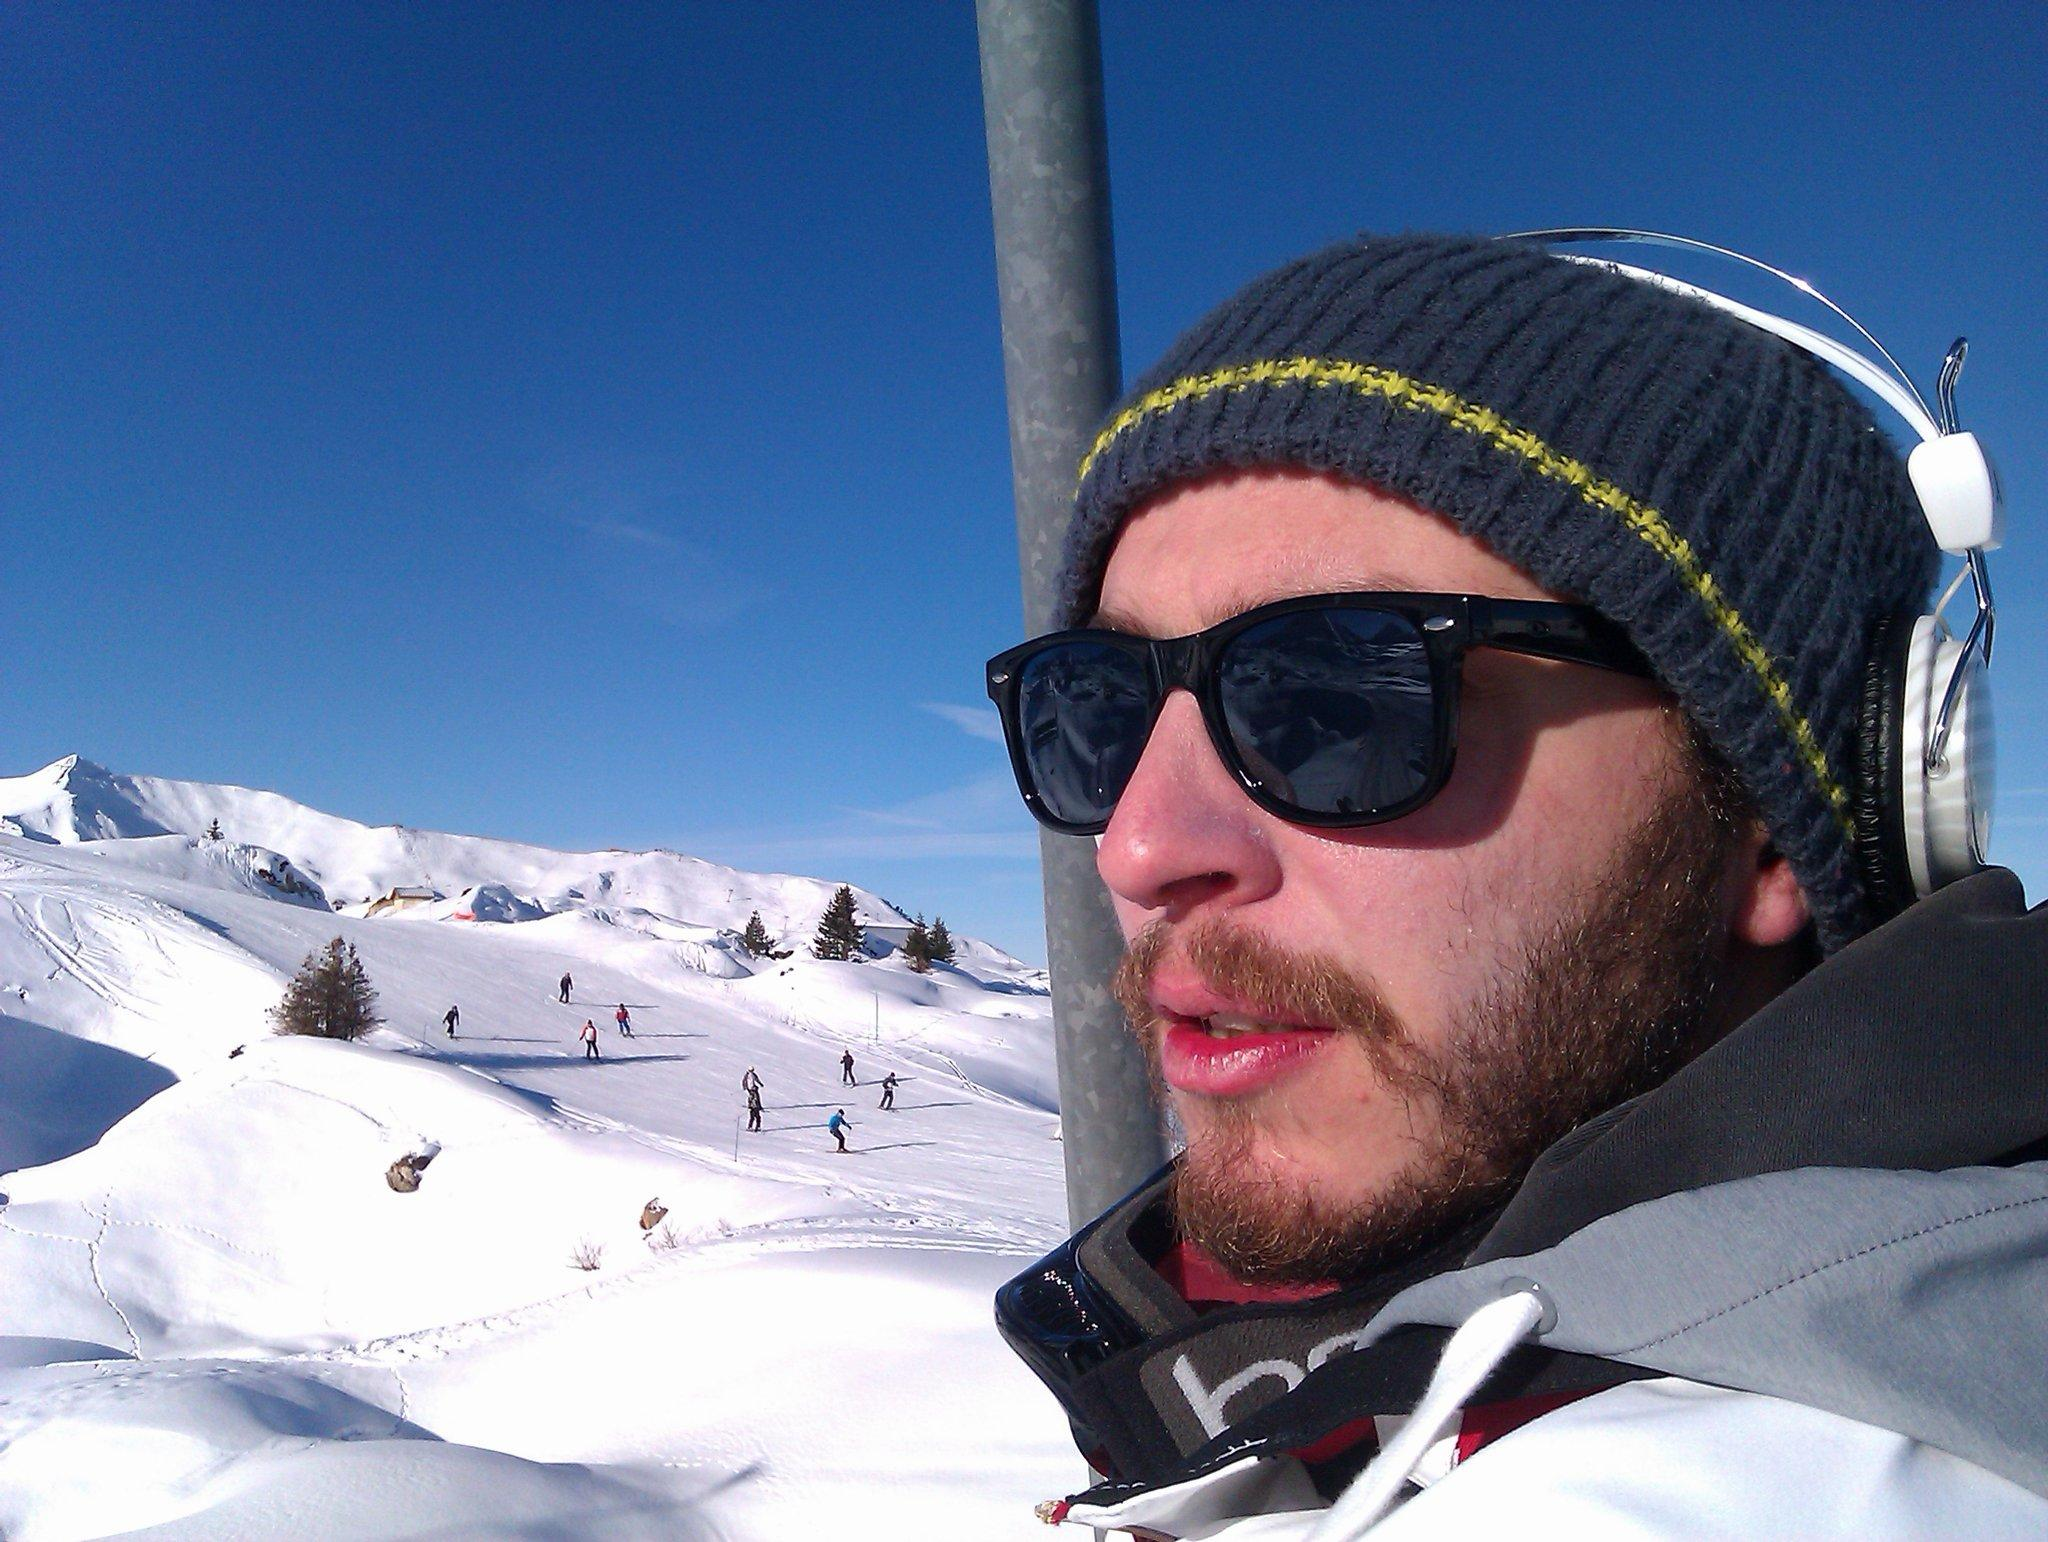
\includegraphics[width=\textwidth]{myself}

    \bigskip

    \tiny Jean-Christophe Loiseau
  \end{minipage}

  \vfill
\end{frame}

%%%%%
%%%%%
%%%%%     INTRODUCTION
%%%%%
%%%%%


\begin{frame}
  \titlepage
\end{frame}

{
  \setbeamercolor*{background canvas}{bg=white}
  \setbeamercolor{normal text}{fg=black}
  \usebeamercolor[fg]{normal text}

  \begin{frame}
    \centering
    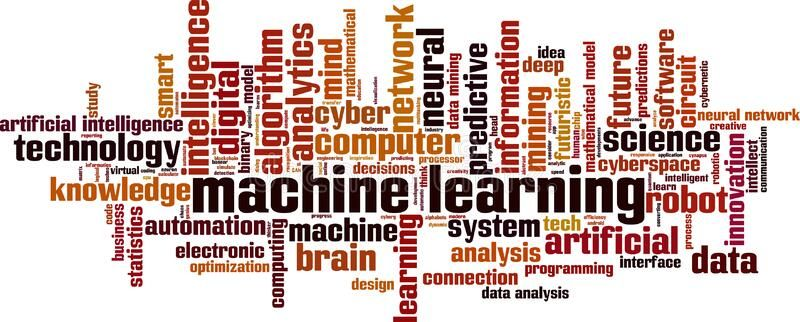
\includegraphics[width=\textwidth]{word_cloud}
  \end{frame}
}

\begin{frame}
  \vfill
  \centering

  \begin{tabular}{p{0.3\textwidth}p{0.66\textwidth}}
    \textbf{\underline{Intelligence Artificielle}} & Ensemble des théories et des techniques développant des programmes informatiques complexes capables de simuler certains traits de l'intelligence humaine (raisonnement, apprentissage, etc).
  \end{tabular}

  \bigskip

  \begin{flushright}
    \small
    Le Petit Robert.
  \end{flushright}
\end{frame}

\begin{frame}
  \centering
  \vfill

  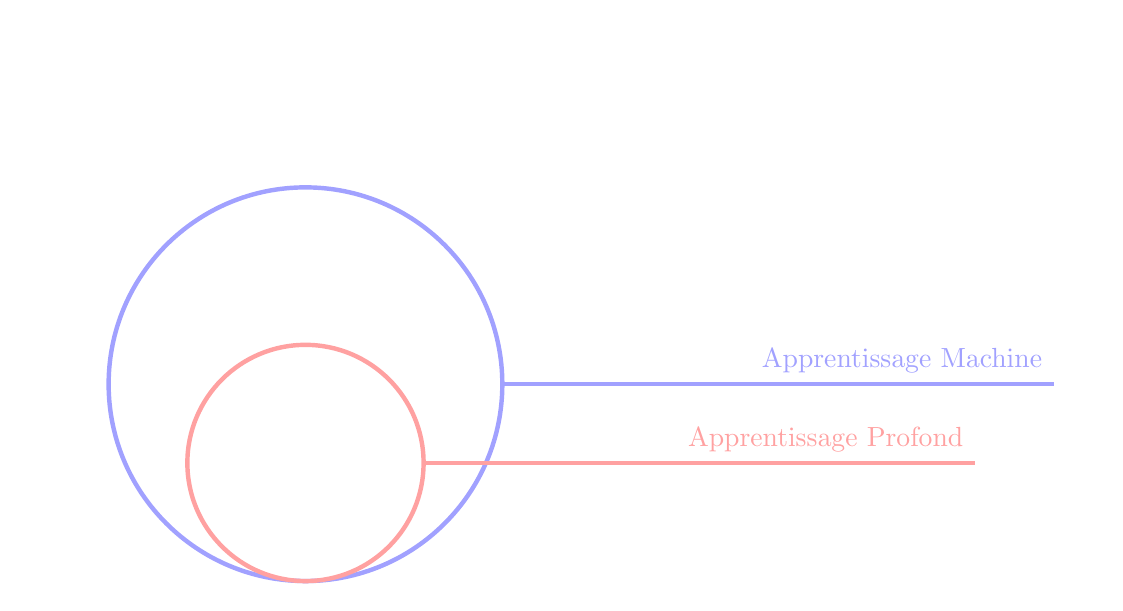
\begin{tikzpicture}
    %\draw[step=1cm, white, very thin] (-7, -4) grid (7,4);

    % AI
    \draw[color=white, ultra thick] (-3, 0) circle (3.5);
    \draw[color=white, ultra thick] (0.5, 0) -- (7, 0) node[above left] {Intelligence Artificielle};

    % Machine Learning
    \draw[color=blue!37, ultra thick] (-3, -1) circle (2.5);
    \draw[color=blue!37, ultra thick] (-0.5, -1) -- (6.5, -1) node[above left] {Apprentissage Machine};

    % Deep Learning
    \draw[color=red!37, ultra thick] (-3, -2) circle (1.5);
    \draw[color=red!37, ultra thick] (-1.5, -2) -- (5.5, -2) node[above left] {Apprentissage Profond};
  \end{tikzpicture}

  \vfill
\end{frame}

\begin{frame}
  \centering
  \vfill

  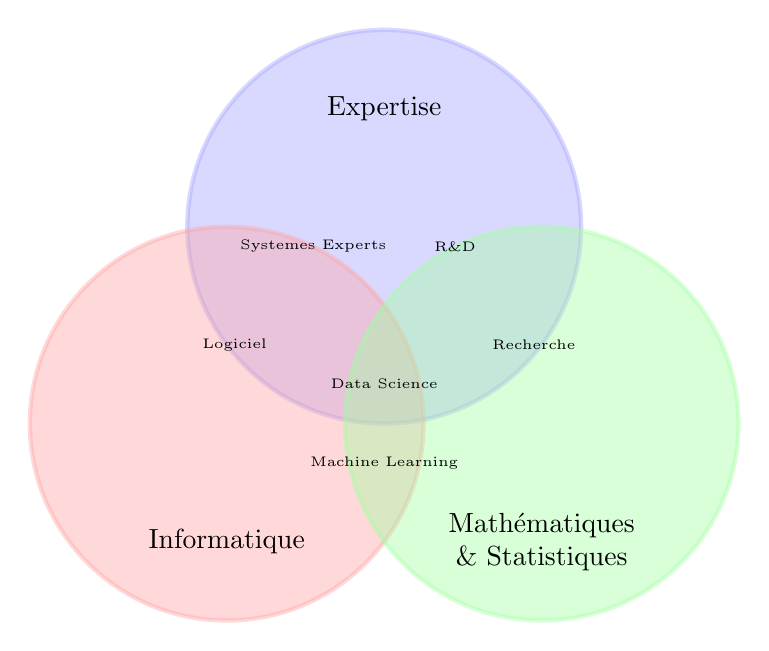
\begin{tikzpicture}
    %\draw[step=1cm, white, very thin] (-7, -4) grid (7,4);

    \draw[color=blue!37, fill=blue!37, opacity=0.4, ultra thick] (0, 1) circle (2.5);
    \draw[color=red!37, fill=red!37, opacity=0.4, ultra thick] (-2, -1.5) circle (2.5);
    \draw[color=green!37, fill=green!37, opacity=0.4, ultra thick] (2, -1.5) circle (2.5);

    \node[align=center] at (0, 2.5) {Expertise};
    \node[align=center] at (2, -3) {Mathématiques \\ \& Statistiques};
    \node[align=center] at (-2, -3) {Informatique};

    \node[align=center] at (0.9, 0.75) {\tiny R\&D};
    \node[align=center] at (1.9, -0.5) {\tiny Recherche};
    \node[align=center] at (-1.9, -0.5) {\tiny Logiciel};
    \node[align=center] at (-0.9, 0.75) {\tiny Systemes Experts};
    \node[align=center] at (0, -1) {\tiny Data Science};
    \node[align=center] at (0, -2) {\tiny Machine Learning};
  
  \end{tikzpicture}

  \vfill
\end{frame}

\begin{frame}
  \vfill
  \centering
  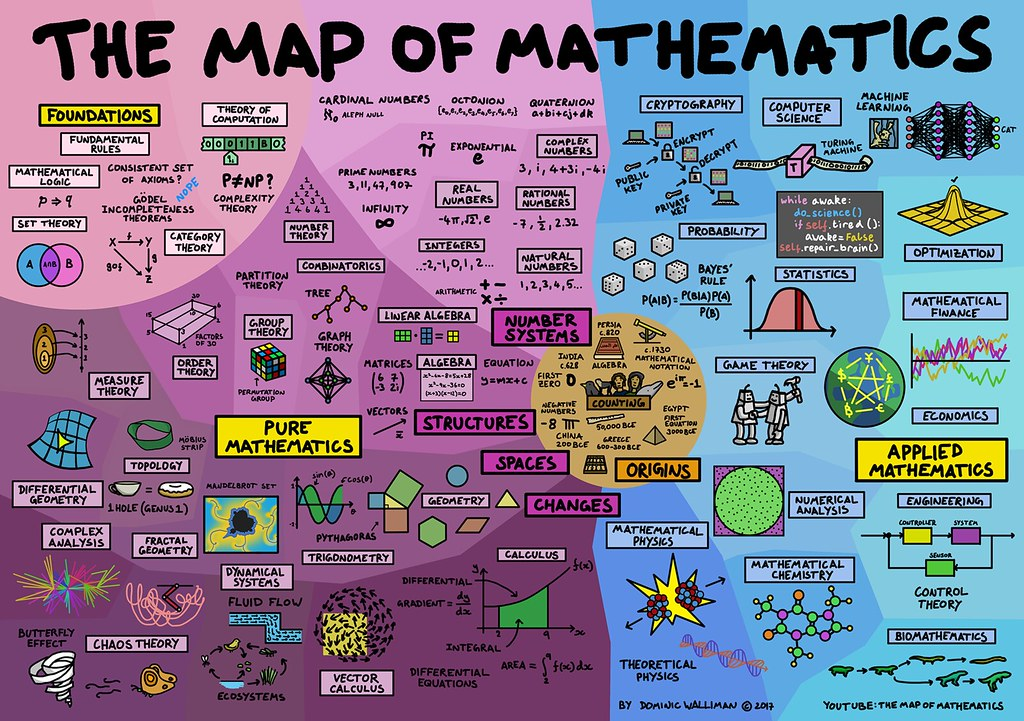
\includegraphics[height=\textheight]{map_of_math}
  \vfill
\end{frame}

{
  \setbeamercolor*{background canvas}{bg=white}
  \setbeamercolor{normal text}{fg=black}
  \usebeamercolor[fg]{normal text}

  \begin{frame}
    \centering
    \vfill
    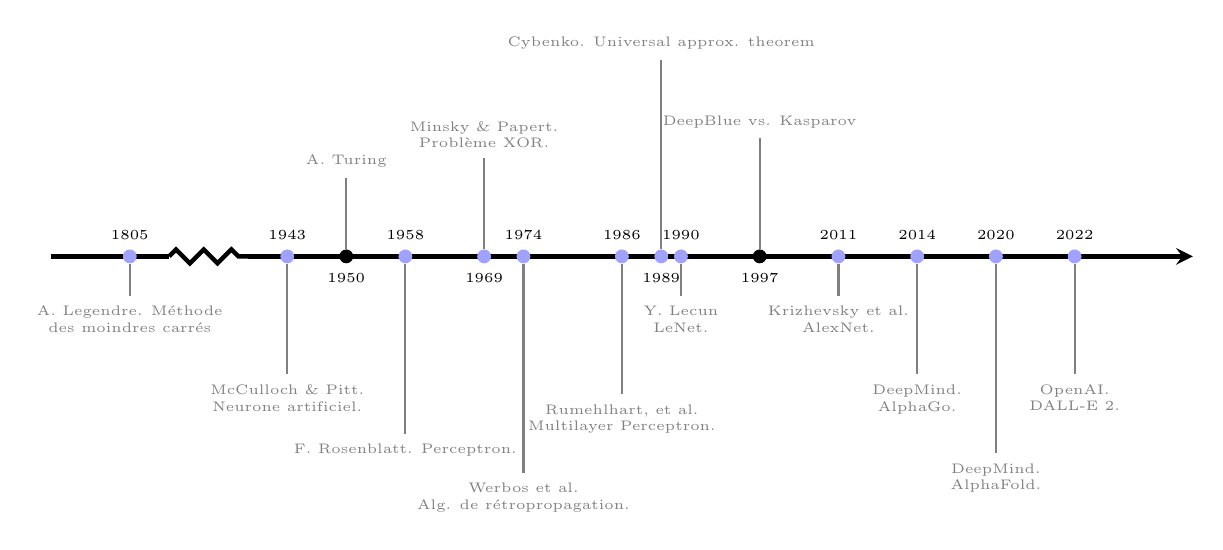
\begin{tikzpicture}[>=stealth]
      %\draw[step=1cm, white, very thin] (-7, -4) grid (7,4);

      % TIMELINE
      \draw[black, ultra thick] (-7.5, 0) -- (-6, 0);
      \draw[black, ultra thick, snake] (-6, 0) -- (-5, 0);
      \draw[black, ultra thick, ->] (-5, 0) -- (7, 0);

      % Legendre & Gauss
      \node[circle, fill=blue!37, inner sep=0pt, minimum size=5pt, label=above:{\tiny 1805}] (lstsq) at (-6.5, 0) {};
      \draw[gray, thick] (lstsq.south) -- (-6.5, -0.5) node[below, align=center, font=\tiny] {A. Legendre. Méthode \\ des moindres carrés};

      % McCullock & Pitt.
      \node[circle, fill=blue!37, inner sep=0pt, minimum size=5pt, label=above:{\tiny 1943}] (neuron) at (-4.5, 0) {};
      \draw[gray, thick] (neuron.south) -- (-4.5, -1.5) node[below, align=center, font=\tiny] {McCulloch \& Pitt. \\ Neurone artificiel.};


      % Alan Turing.
      \node[circle, fill=black, inner sep=0pt, minimum size=5pt, label=below:{\tiny 1950}] (turing) at (-3.75, 0) {};
      \draw[gray, thick] (turing.north) -- (-3.75, 1) node[above, align=center, font=\tiny] {A. Turing};

      % F. Rosenblatt.
      \node[circle, fill=blue!37, inner sep=0pt, minimum size=5pt, label=above:{\tiny 1958}] (rosenblatt) at (-3, 0) {};
      \draw[gray, thick] (rosenblatt.south) -- (-3, -2.25) node[below, align=center, font=\tiny] {F. Rosenblatt. Perceptron.};

      % XOR
      \node[circle, fill=blue!37, inner sep=0pt, minimum size=5pt, label=below:{\tiny 1969}] (xor) at (-2, 0) {};
      \draw[gray, thick] (xor.north) -- (-2, 1.25) node[above, align=center, font=\tiny] {Minsky \& Papert. \\ Problème XOR.};

      % Backpropagation.
      \node[circle, fill=blue!37, inner sep=0pt, minimum size=5pt, label=above:{\tiny 1974}] (backprop) at (-1.5, 0) {};
      \draw[gray, thick] (backprop.south) -- (-1.5, -2.75) node[below, align=center, font=\tiny] {Werbos et al. \\ Alg. de rétropropagation.};

      % MLP.
      \node[circle, fill=blue!37, inner sep=0pt, minimum size=5pt, label=above:{\tiny 1986}] (mlp) at (-0.25, 0) {};
      \draw[gray, thick] (mlp.south) -- (-0.25, -1.75) node[below, align=center, font=\tiny] {Rumehlhart, et al. \\ Multilayer Perceptron.};

      % Cybenko.
      \node[circle, fill=blue!37, inner sep=0pt, minimum size=5pt, label=below:{\tiny 1989}] (lenet) at (0.25, 0) {};
      \draw[gray, thick] (lenet.north) -- (0.25, 2.5) node[above, align=center, font=\tiny] {Cybenko. Universal approx. theorem};


      % LeNet.
      \node[circle, fill=blue!37, inner sep=0pt, minimum size=5pt, label=above:{\tiny 1990}] (lenet) at (0.5, 0) {};
      \draw[gray, thick] (lenet.south) -- (0.5, -0.5) node[below, align=center, font=\tiny] {Y. Lecun \\ LeNet.};

      % DeepBlue.
      \node[circle, fill=black, inner sep=0pt, minimum size=5pt, label=below:{\tiny 1997}] (deepblue) at (1.5, 0) {};
      \draw[gray, thick] (deepblue.north) -- (1.5, 1.5) node[above, align=center, font=\tiny] {DeepBlue vs. Kasparov};

      % AlexNet.
      \node[circle, fill=blue!37, inner sep=0pt, minimum size=5pt, label=above:{\tiny 2011}] (alexnet) at (2.5, 0) {};
      \draw[gray, thick] (alexnet.south) -- (2.5, -0.5) node[below, align=center, font=\tiny] {Krizhevsky et al. \\ AlexNet.};

      % AlphaGo
      \node[circle, fill=blue!37, inner sep=0pt, minimum size=5pt, label=above:{\tiny 2014}] (alphago) at (3.5, 0) {};
      \draw[gray, thick] (alphago.south) -- (3.5, -1.5) node[below, align=center, font=\tiny] {DeepMind. \\ AlphaGo.};

      % AlphaFold
      \node[circle, fill=blue!37, inner sep=0pt, minimum size=5pt, label=above:{\tiny 2020}] (alphafold) at (4.5, 0) {};
      \draw[gray, thick] (alphafold.south) -- (4.5, -2.5) node[below, align=center, font=\tiny] {DeepMind. \\ AlphaFold.};

      % Dalle-e
      \node[circle, fill=blue!37, inner sep=0pt, minimum size=5pt, label=above:{\tiny 2022}] (dalle) at (5.5, 0) {};
      \draw[gray, thick] (dalle.south) -- (5.5, -1.5) node[below, align=center, font=\tiny] {OpenAI. \\ DALL-E 2.};
    \end{tikzpicture}

    \vfill
  \end{frame}

  \begin{frame}
    \centering
    \vfill
    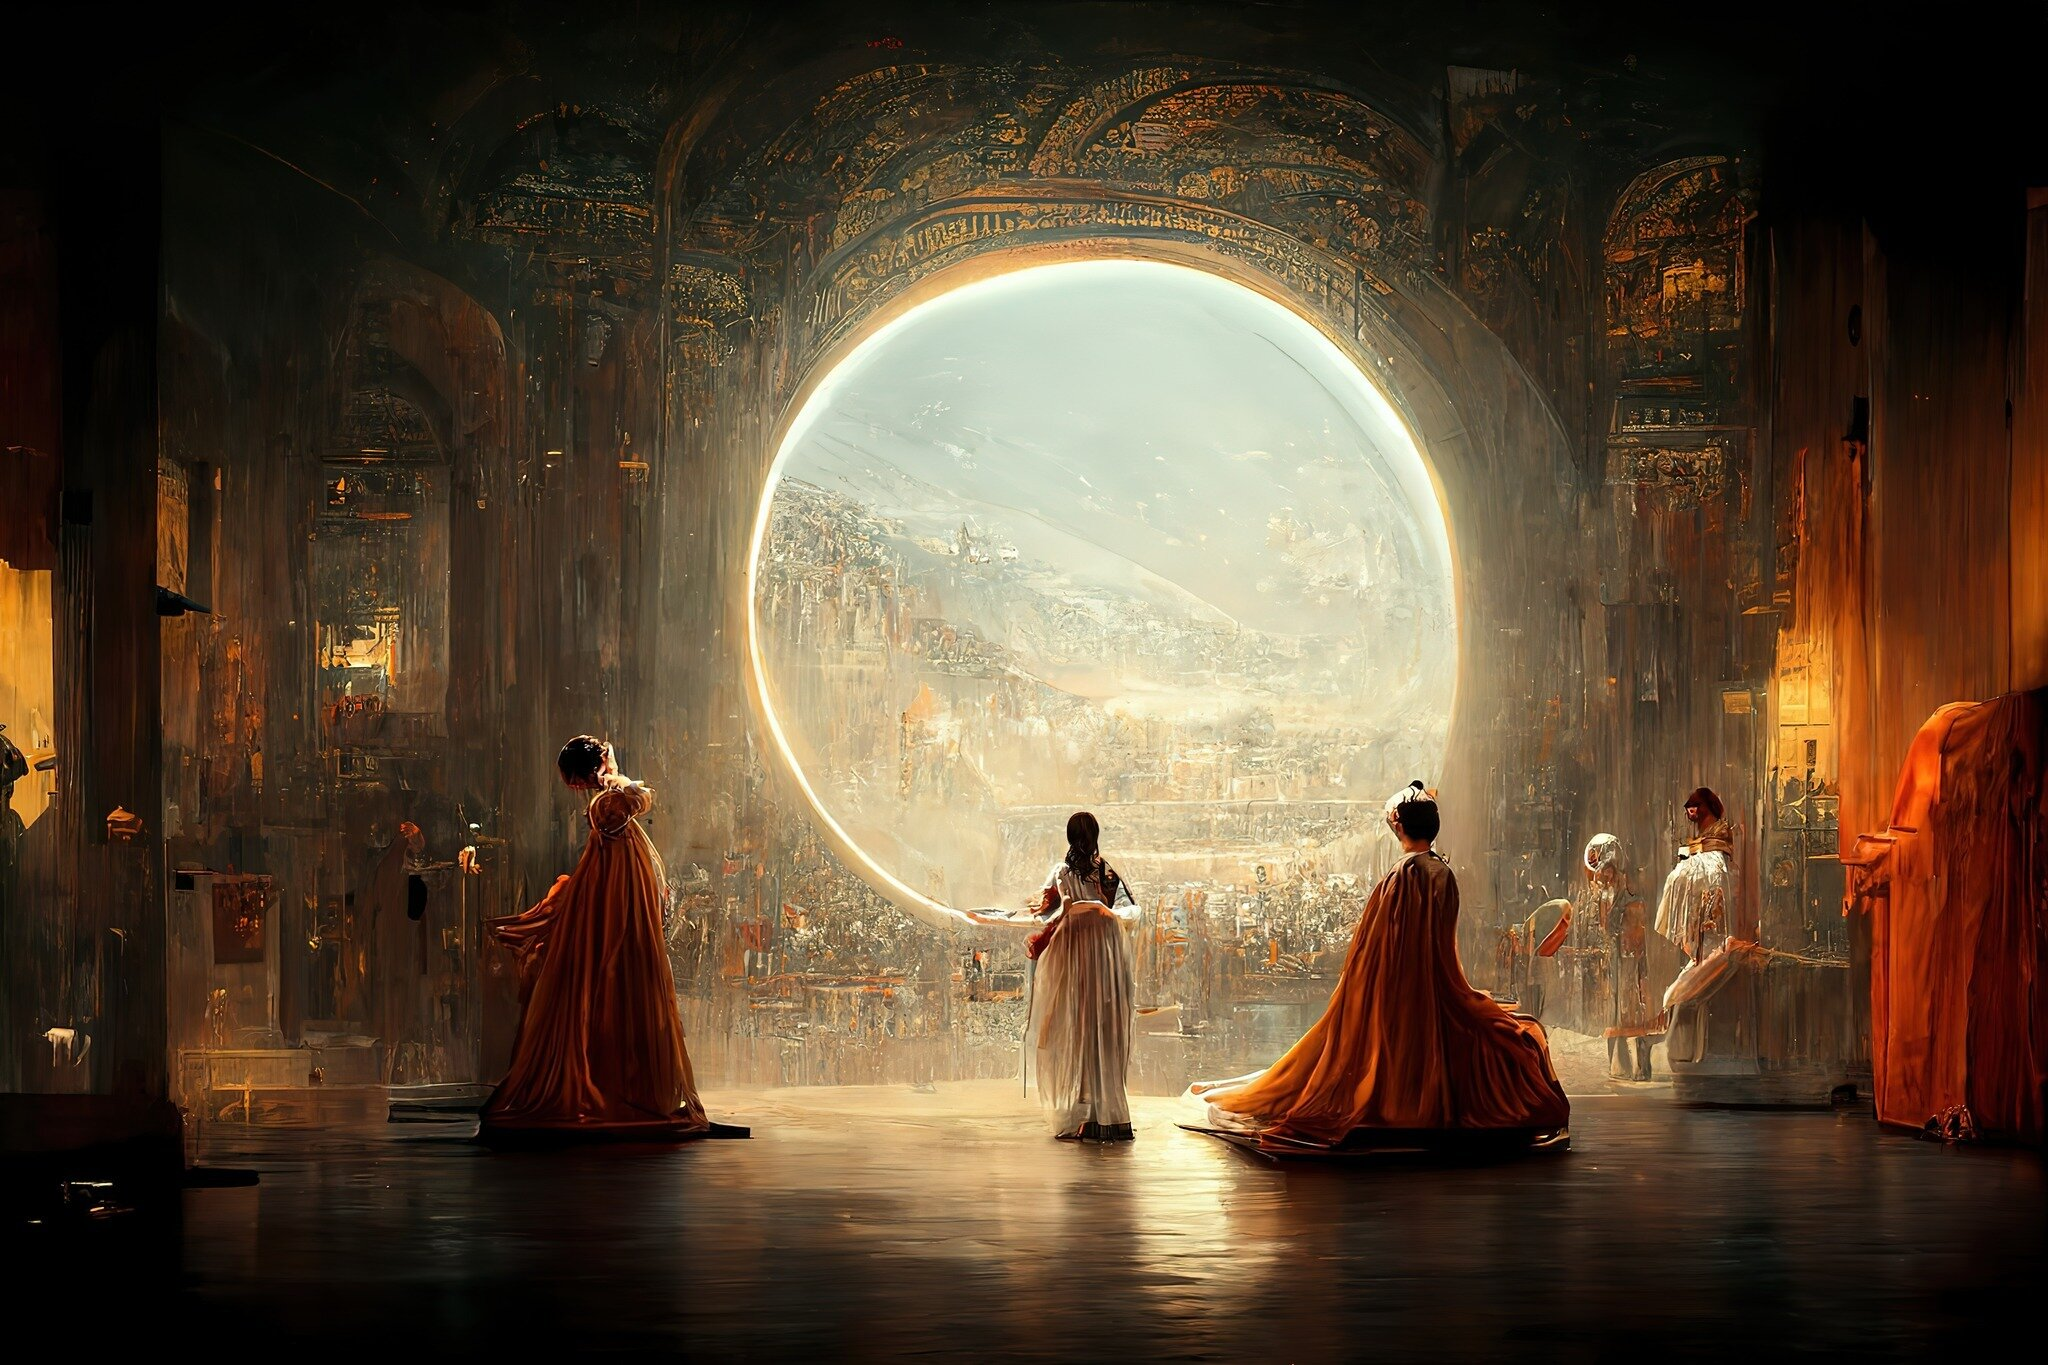
\includegraphics[height=\textheight]{ai_art}
    \vfill
  \end{frame}

}

\section{Un réseau de neurones, qu'est ce que c'est ?}
\begin{frame}
  \sectionpage
\end{frame}

{
  \setbeamercolor*{background canvas}{bg=white}
  \setbeamercolor{normal text}{fg=black}
  \usebeamercolor[fg]{normal text}
  
  \begin{frame}
    \centering
    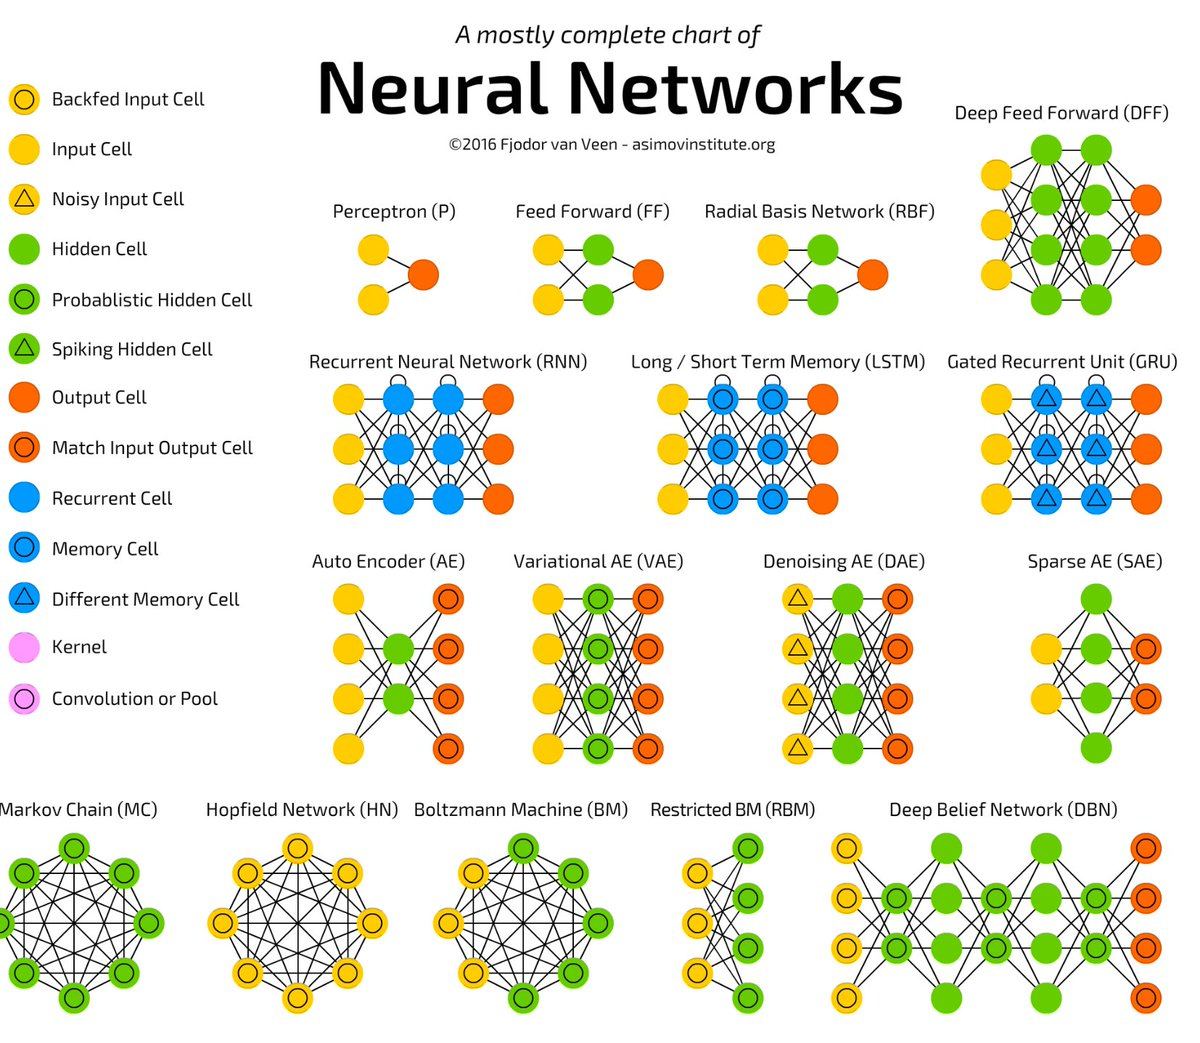
\includegraphics[height=\textheight]{neuralnet_zoo}
  \end{frame}

  \begin{frame}
    \centering
    \vfill
    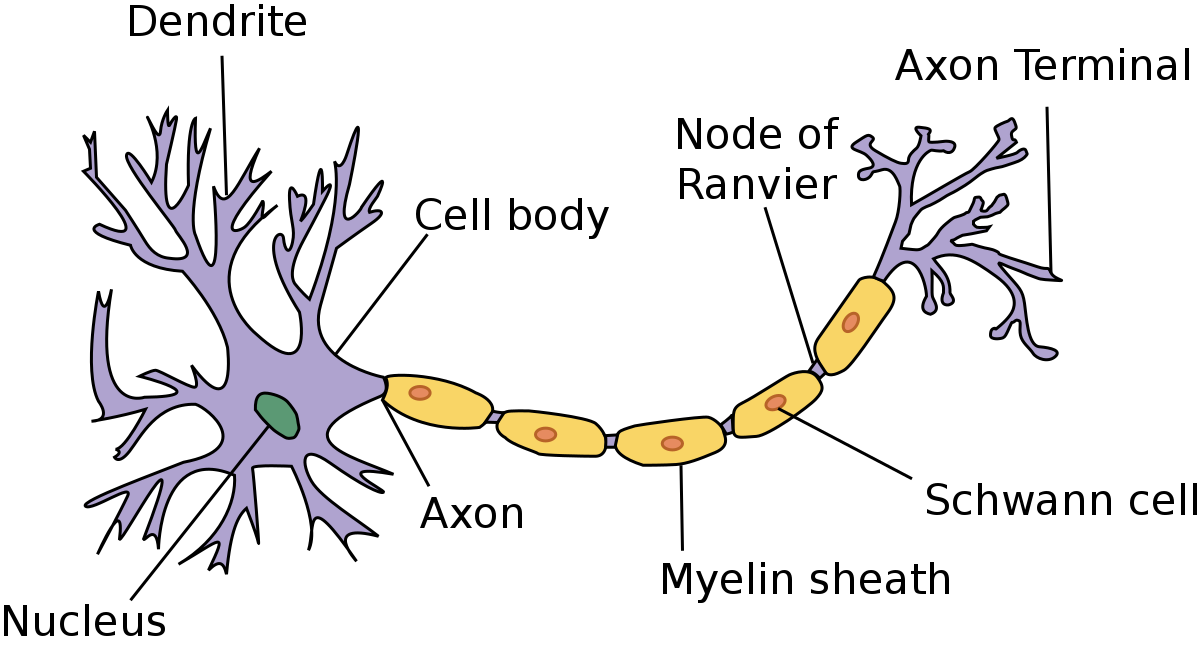
\includegraphics[height=.65\textheight]{neuron}
    \vfill
  \end{frame}

}

\begin{frame}
  \centering
  \vfill
  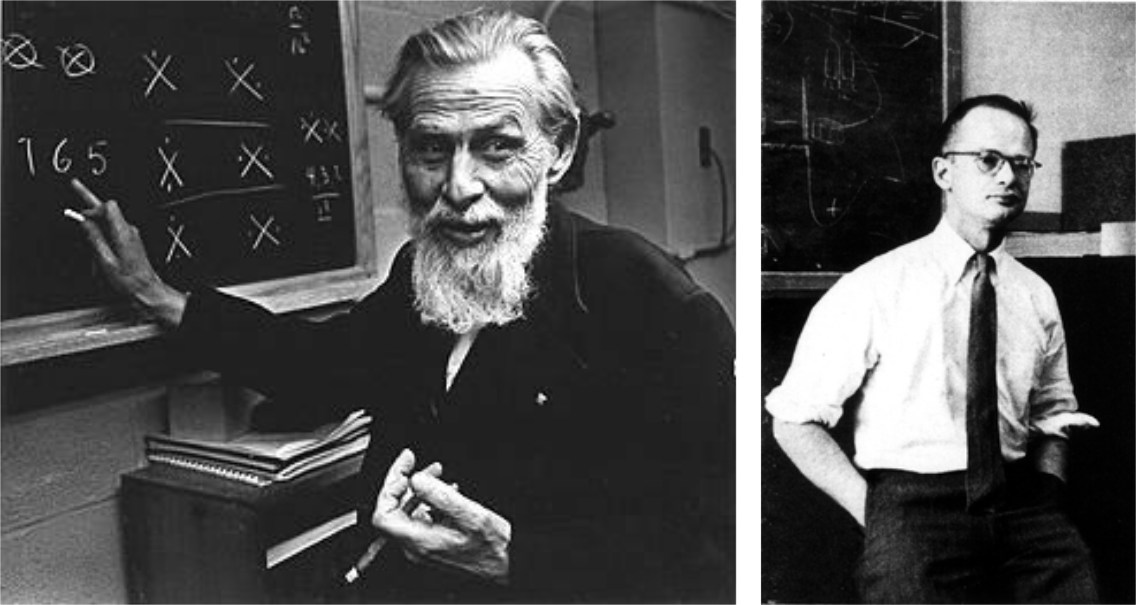
\includegraphics[height=.65\textheight]{McCulloch_Pitts}

  \bigskip

  {\tiny
    McCulloch \& Pitts. \emph{A logical calculus of the ideas immanent in nervous activity}. 1943.
  }
  \vfill
\end{frame}

\begin{frame}
  \centering
  \vfill
  \begin{tikzpicture}[>=stealth]
    %\draw[step=1cm, white, very thin] (-7, -4) grid (7,4);

    \node[left] (input1) at (-5, 3) {$x_1$};
    \node[left] (input2) at (-5, 2) {$x_2$};
    \node[left] (input3) at (-5, 1) {$x_3$};
    \node[left] (input4) at (-5, 0) {$x_4$};
    \node[left] (input5) at (-5, -1) {$x_5$};
    \node[left] (input6) at (-5, -2) {$x_6$};
    \node[left] (input7) at (-5, -3) {$x_7$};

    \node[circle, draw=white, ultra thick, font=\small, label=below:{Neurone MCP}] (mcp) at (1, 0) {
      $
      \sigma(\bm{x})
      =
      \begin{cases}
        1 \quad \textrm{si} \quad \sum x_i \geq b\\
        0 \quad \textrm{sinon.}
      \end{cases}
      $
    };

    \draw[->, ultra thick, white] (mcp.east) -- (6, 0) node[right] {$y \in \left\{ 0, 1 \right\}$};

    \draw[ultra thick, white] (input1.east) -- (mcp.west);
    \draw[ultra thick, white] (input2.east) -- (mcp.west);
    \draw[ultra thick, white] (input3.east) -- (mcp.west);
    \draw[ultra thick, white] (input4.east) -- (mcp.west);
    \draw[ultra thick, white] (input5.east) -- (mcp.west);
    \draw[ultra thick, white] (input6.east) -- (mcp.west);
    \draw[ultra thick, white] (input7.east) -- (mcp.west);

  \end{tikzpicture}
  \vfill
\end{frame}

\begin{frame}
  \vfill
  \centering

  \underline{Algèbre Booléenne avec des neurones MCP}

  \vfill

  \begin{minipage}{.48\textwidth}
    \centering
    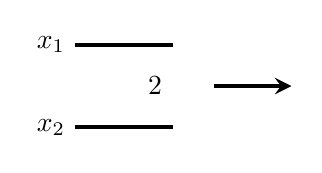
\begin{tikzpicture}[>=stealth]
      
      \node[circle split, ultra thick, draw=white, rotate=90] (mcp) at (0, 0) {\rotatebox{-90}{2}};
      \node[left=1.25cm of mcp.east] (input1) {$x_1$};
      \node[left=1.25cm of mcp.west] (input2) {$x_2$};

      \draw[->, ultra thick] (mcp.south) -- (1.5, 0);
      \draw[ultra thick] (input1.east) -- (mcp.east);
      \draw[ultra thick] (input2.east) -- (mcp.west);
    \end{tikzpicture}

    \bigskip

    AND
  \end{minipage}%
  \hfill
  \begin{minipage}{.48\textwidth}
    \centering
    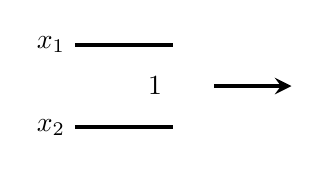
\begin{tikzpicture}[>=stealth]
      
      \node[circle split, ultra thick, draw=white, rotate=90] (mcp) at (0, 0) {\rotatebox{-90}{1}};
      \node[left=1.25cm of mcp.east] (input1) {$x_1$};
      \node[left=1.25cm of mcp.west] (input2) {$x_2$};

      \draw[->, ultra thick] (mcp.south) -- (1.5, 0);
      \draw[ultra thick] (input1.east) -- (mcp.east);
      \draw[ultra thick] (input2.east) -- (mcp.west);

    \end{tikzpicture}

    \bigskip

    OR
  \end{minipage}
  \vfill
\end{frame}

\begin{frame}
  \vfill
  \centering
  \begin{minipage}{.48\textwidth}
    \centering
    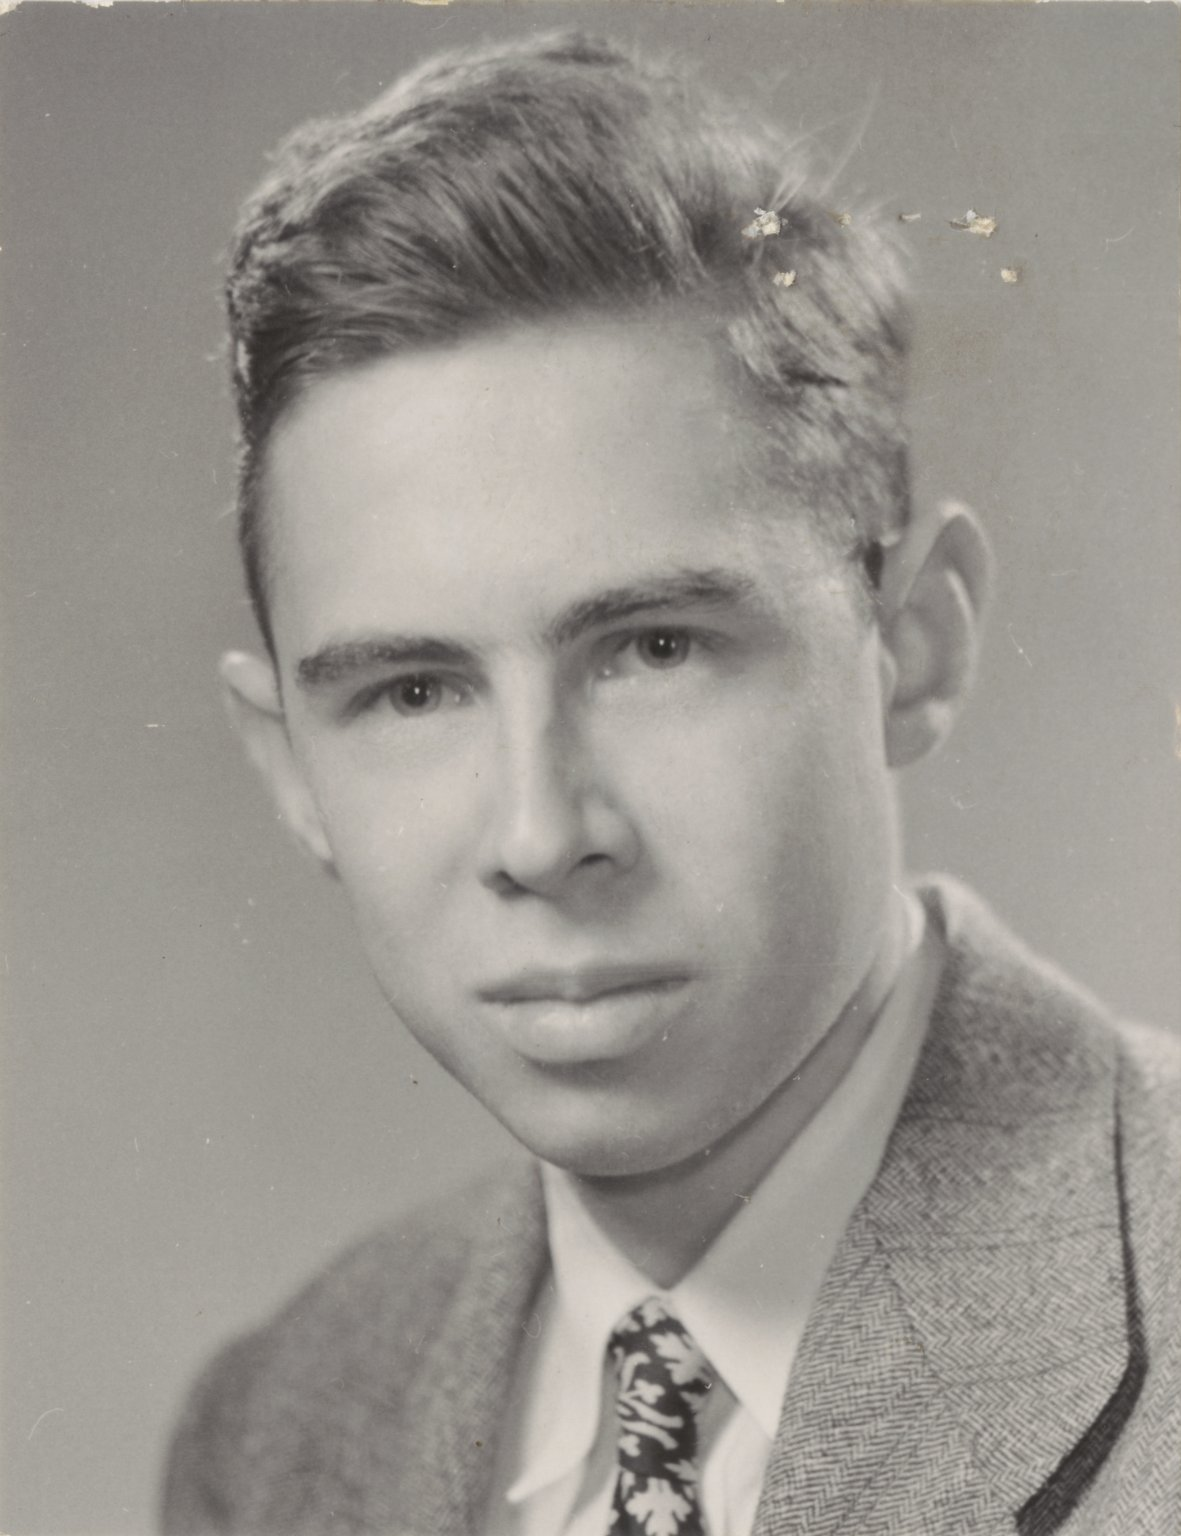
\includegraphics[height=.6\textheight]{Rosenblatt_21}
  \end{minipage}%
  \hfill
  \begin{minipage}{.48\textwidth}
    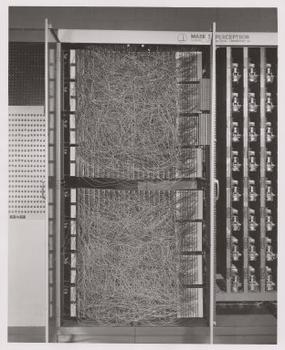
\includegraphics[height=.6\textheight]{Mark_I_perceptron}
  \end{minipage}

  \bigskip

  {\tiny
    F. Rosenblatt. \emph{The Perceptron -- a perceiving and recognizing automaton}. 1957.
  }

  \vfill
\end{frame}


\begin{frame}
  \centering
  \vfill
  \begin{tikzpicture}[>=stealth]
    %\draw[step=1cm, white, very thin] (-7, -4) grid (7,4);

    \node[left] (input1) at (-5, 3) {$x_1$};
    \node[left] (input2) at (-5, 2) {$x_2$};
    \node[left] (input3) at (-5, 1) {$x_3$};
    \node[left] (input4) at (-5, 0) {$x_4$};
    \node[left] (input5) at (-5, -1) {$x_5$};
    \node[left] (input6) at (-5, -2) {$x_6$};
    \node[left] (input7) at (-5, -3) {$x_7$};

    \node[circle, draw=white, ultra thick, font=\small, label=below:{Neurone artificiel}] (mcp) at (1, 0) {
      $
      \sigma(\bm{x})
      =
      \begin{cases}
        1 \quad \textrm{si} \quad \sum {\color{red}w_i} x_i + b \geq 0\\
        0 \quad \textrm{sinon.}
      \end{cases}
      $
    };

    \draw[->, ultra thick, white] (mcp.east) -- (6, 0) node[right] {$y \in \left\{ 0, 1 \right\}$};

    \draw[ultra thick, white] (input1.east) -- (mcp.west);
    \draw[ultra thick, white] (input2.east) -- (mcp.west);
    \draw[ultra thick, white] (input3.east) -- (mcp.west);
    \draw[ultra thick, white] (input4.east) -- (mcp.west);
    \draw[ultra thick, white] (input5.east) -- (mcp.west);
    \draw[ultra thick, white] (input6.east) -- (mcp.west);
    \draw[ultra thick, white] (input7.east) -- (mcp.west);

  \end{tikzpicture}
  \vfill
\end{frame}

\begin{frame}[fragile]{}{}
  \begin{algorithm}[H]
    \DontPrintSemicolon

    \KwInput{Le jeu d'entraînement $\left\{ \bm{x}_i, y_i \right\}$, le taux d'apprentissage $\alpha$.}
    \KwOutput{Les paramètres $\left( \bm{w}, b \right)$ du perceptron.}

    Initialiser $\bm{w}$ and $b$ aléatoirement.% \tcp*{Initialize the set $Z$ to be the empty set.}

    \While{not converged}{
      \For{$k = 1, \cdots, n$}{

        $\varepsilon = y_i - \sigma(\bm{w}^T \bm{x}_i + b)$

        \If{$\varepsilon \neq 0$}{
          $\bm{w} = \bm{w} + \alpha \varepsilon \bm{x}_i$

          $b = b + \alpha \varepsilon$
        }
      }

      Test de la convergence.
    }

    \caption{\small Perceptron Learning Algorithm}
    \label{alg: naive greedy algorithm}
  \end{algorithm}
\end{frame}

\begin{frame}
  \vfill
  \centering

  \underline{\textbf{Démonstration sur MNIST}}

  \vfill

  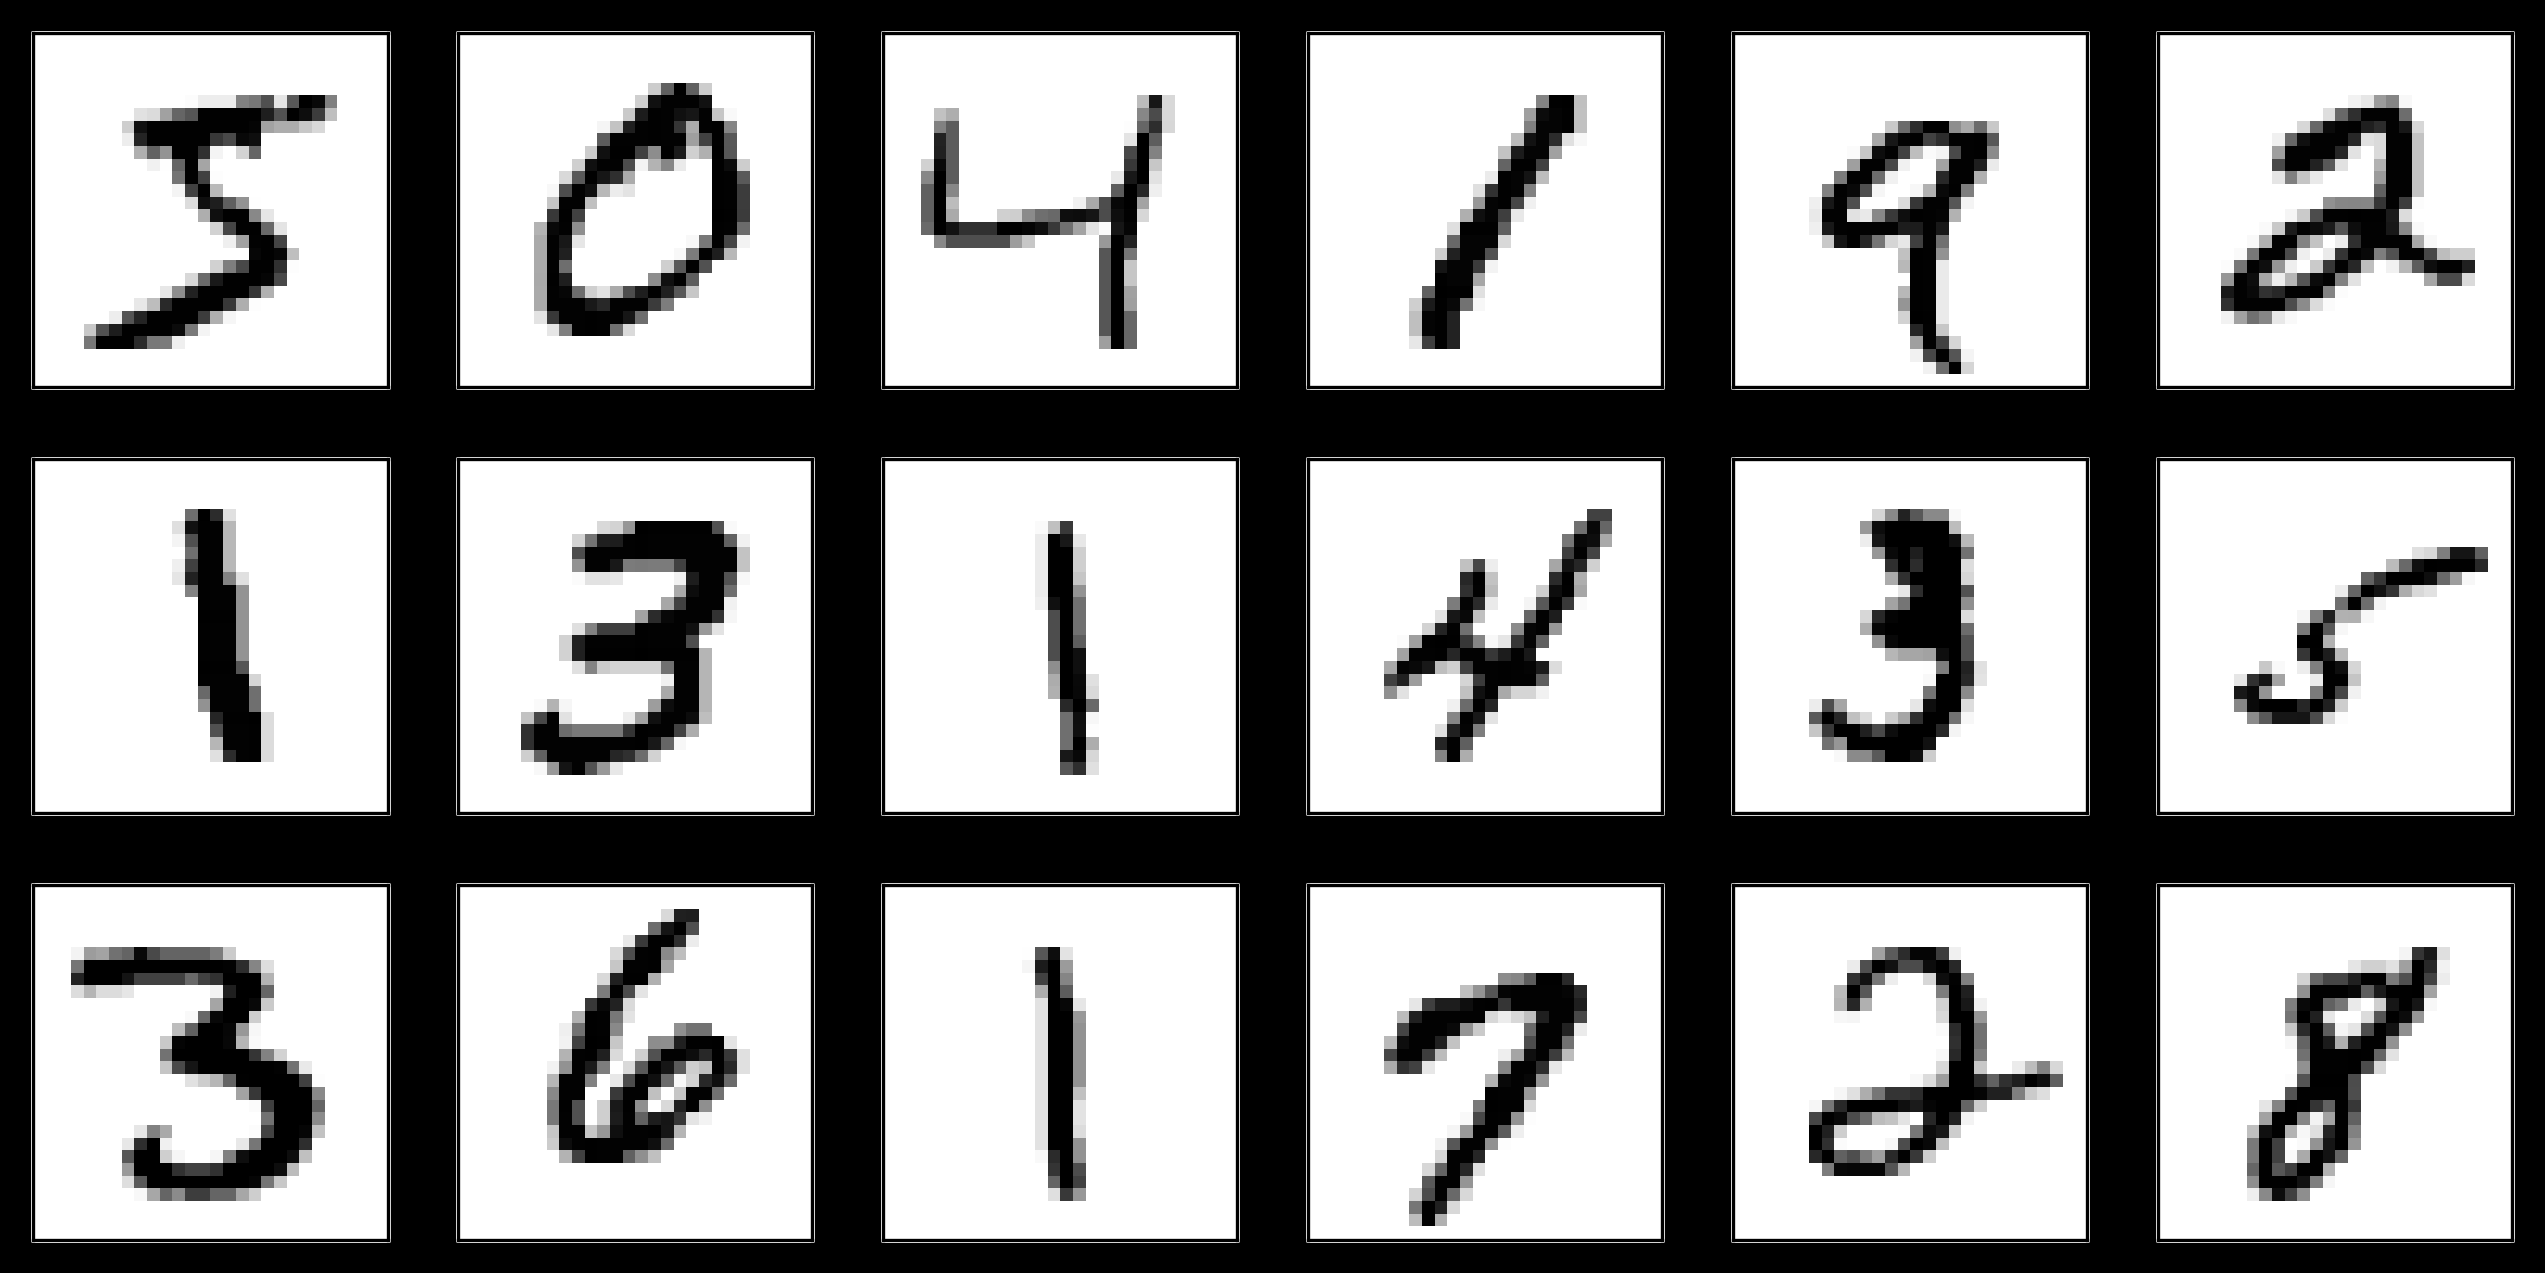
\includegraphics[height=.5\textheight]{MNIST}

  \vfill
\end{frame}

\begin{frame}
  \centering
  \vfill

  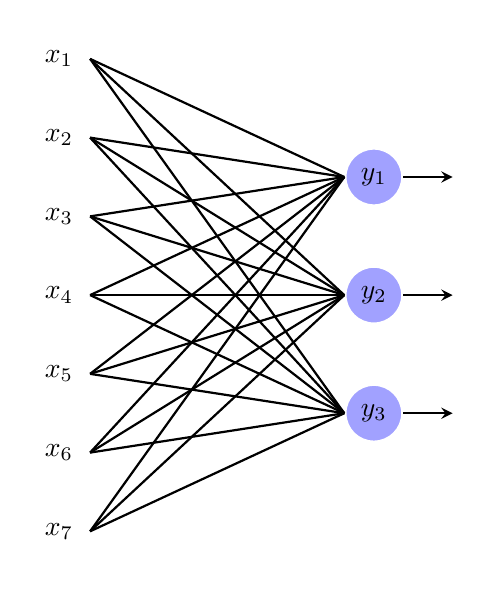
\begin{tikzpicture}[>=stealth]
    %\draw[step=1cm, white, very thin] (-7, -4) grid (7,4);

    \node[circle, draw=white, ultra thick] (in1) at (-2, 3) {$x_1$};
    \node[circle, draw=white, ultra thick] (in2) at (-2, 2) {$x_2$};
    \node[circle, draw=white, ultra thick] (in3) at (-2, 1) {$x_3$};
    \node[circle, draw=white, ultra thick] (in4) at (-2, 0) {$x_4$};
    \node[circle, draw=white, ultra thick] (in5) at (-2, -1) {$x_5$};
    \node[circle, draw=white, ultra thick] (in6) at (-2, -2) {$x_6$};
    \node[circle, draw=white, ultra thick] (in7) at (-2, -3) {$x_7$};

    \node[circle, draw=white, fill=blue!37, thick] (out1) at (2, 1.5) {$y_1$};
    \node[circle, draw=white, fill=blue!37, thick] (out2) at (2, 0) {$y_2$};
    \node[circle, draw=white, fill=blue!37, thick] (out3) at (2, -1.5) {$y_3$};

    \draw[thick] (in1.east) -- (out1.west);
    \draw[thick] (in1.east) -- (out2.west);
    \draw[thick] (in1.east) -- (out3.west);

    \draw[thick] (in2.east) -- (out1.west);
    \draw[thick] (in2.east) -- (out2.west);
    \draw[thick] (in2.east) -- (out3.west);

    \draw[thick] (in3.east) -- (out1.west);
    \draw[thick] (in3.east) -- (out2.west);
    \draw[thick] (in3.east) -- (out3.west);

    \draw[thick] (in4.east) -- (out1.west);
    \draw[thick] (in4.east) -- (out2.west);
    \draw[thick] (in4.east) -- (out3.west);

    \draw[thick] (in5.east) -- (out1.west);
    \draw[thick] (in5.east) -- (out2.west);
    \draw[thick] (in5.east) -- (out3.west);

    \draw[thick] (in6.east) -- (out1.west);
    \draw[thick] (in6.east) -- (out2.west);
    \draw[thick] (in6.east) -- (out3.west);

    \draw[thick] (in7.east) -- (out1.west);
    \draw[thick] (in7.east) -- (out2.west);
    \draw[thick] (in7.east) -- (out3.west);

    \draw[thick, ->] (out1.east) -- (3, 1.5);
    \draw[thick, ->] (out2.east) -- (3, 0);
    \draw[thick, ->] (out3.east) -- (3, -1.5);

  \end{tikzpicture}

  \vfill
\end{frame}

\begin{frame}
  \centering
  \vfill
  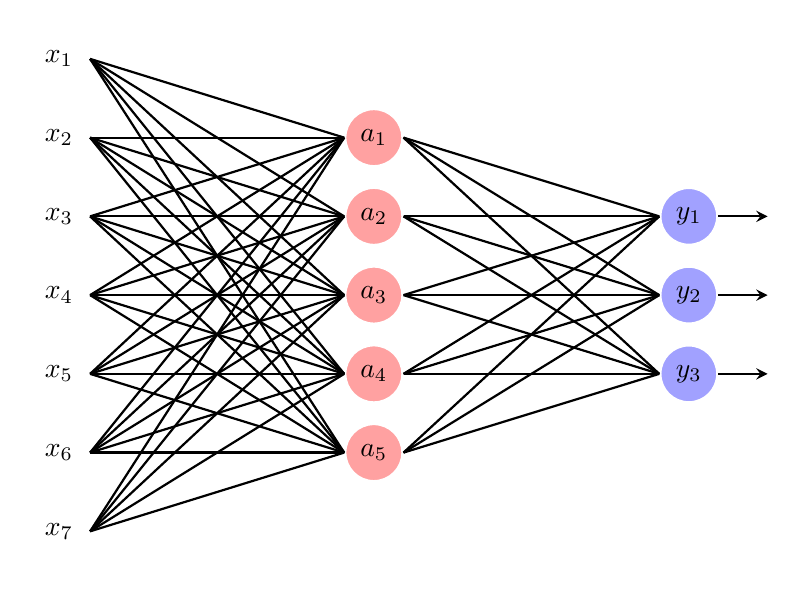
\begin{tikzpicture}[>=stealth]
    \node[circle, draw=white, ultra thick] (in1) at (-2, 3) {$x_1$};
    \node[circle, draw=white, ultra thick] (in2) at (-2, 2) {$x_2$};
    \node[circle, draw=white, ultra thick] (in3) at (-2, 1) {$x_3$};
    \node[circle, draw=white, ultra thick] (in4) at (-2, 0) {$x_4$};
    \node[circle, draw=white, ultra thick] (in5) at (-2, -1) {$x_5$};
    \node[circle, draw=white, ultra thick] (in6) at (-2, -2) {$x_6$};
    \node[circle, draw=white, ultra thick] (in7) at (-2, -3) {$x_7$};

    \node[circle, draw=white, thick, fill=red!37] (hid1) at (2, 2) {$a_1$};
    \node[circle, draw=white, thick, fill=red!37] (hid2) at (2, 1) {$a_2$};
    \node[circle, draw=white, thick, fill=red!37] (hid3) at (2, 0) {$a_3$};
    \node[circle, draw=white, thick, fill=red!37] (hid4) at (2, -1) {$a_4$};
    \node[circle, draw=white, thick, fill=red!37] (hid5) at (2, -2) {$a_5$};

    \node[circle, draw=white, fill=blue!37, thick] (out1) at (6, 1) {$y_1$};
    \node[circle, draw=white, fill=blue!37, thick] (out2) at (6, 0) {$y_2$};
    \node[circle, draw=white, fill=blue!37, thick] (out3) at (6, -1) {$y_3$};

    \draw[thick, ->] (out1.east) -- (7, 1);
    \draw[thick, ->] (out2.east) -- (7, 0);
    \draw[thick, ->] (out3.east) -- (7, -1);

    \draw[thick] (in1.east) -- (hid1.west);
    \draw[thick] (in1.east) -- (hid2.west);
    \draw[thick] (in1.east) -- (hid3.west);
    \draw[thick] (in1.east) -- (hid4.west);
    \draw[thick] (in1.east) -- (hid5.west);

    \draw[thick] (in2.east) -- (hid1.west);
    \draw[thick] (in2.east) -- (hid2.west);
    \draw[thick] (in2.east) -- (hid3.west);
    \draw[thick] (in2.east) -- (hid4.west);
    \draw[thick] (in2.east) -- (hid5.west);

    \draw[thick] (in3.east) -- (hid1.west);
    \draw[thick] (in3.east) -- (hid2.west);
    \draw[thick] (in3.east) -- (hid3.west);
    \draw[thick] (in3.east) -- (hid4.west);
    \draw[thick] (in3.east) -- (hid5.west);

    \draw[thick] (in4.east) -- (hid1.west);
    \draw[thick] (in4.east) -- (hid2.west);
    \draw[thick] (in4.east) -- (hid3.west);
    \draw[thick] (in4.east) -- (hid4.west);
    \draw[thick] (in4.east) -- (hid5.west);

    \draw[thick] (in5.east) -- (hid1.west);
    \draw[thick] (in5.east) -- (hid2.west);
    \draw[thick] (in5.east) -- (hid3.west);
    \draw[thick] (in5.east) -- (hid4.west);
    \draw[thick] (in5.east) -- (hid5.west);

    \draw[thick] (in6.east) -- (hid1.west);
    \draw[thick] (in6.east) -- (hid2.west);
    \draw[thick] (in6.east) -- (hid3.west);
    \draw[thick] (in6.east) -- (hid4.west);
    \draw[thick] (in6.east) -- (hid5.west);

    \draw[thick] (in7.east) -- (hid1.west);
    \draw[thick] (in7.east) -- (hid2.west);
    \draw[thick] (in7.east) -- (hid3.west);
    \draw[thick] (in7.east) -- (hid4.west);
    \draw[thick] (in7.east) -- (hid5.west);

    \draw[thick] (hid1.east) -- (out1.west);
    \draw[thick] (hid1.east) -- (out2.west);
    \draw[thick] (hid1.east) -- (out3.west);

    \draw[thick] (hid2.east) -- (out1.west);
    \draw[thick] (hid2.east) -- (out2.west);
    \draw[thick] (hid2.east) -- (out3.west);

    \draw[thick] (hid3.east) -- (out1.west);
    \draw[thick] (hid3.east) -- (out2.west);
    \draw[thick] (hid3.east) -- (out3.west);

    \draw[thick] (hid4.east) -- (out1.west);
    \draw[thick] (hid4.east) -- (out2.west);
    \draw[thick] (hid4.east) -- (out3.west);

    \draw[thick] (hid5.east) -- (out1.west);
    \draw[thick] (hid5.east) -- (out2.west);
    \draw[thick] (hid5.east) -- (out3.west);

  \end{tikzpicture}
  \vfill
\end{frame}

%% \begin{frame}
%%   \centering
%%   \vfill
%%   Démonstration du Perceptron en Python.
%%   \vfill
%% \end{frame}

%% {
%%   \setbeamercolor*{background canvas}{bg=white}
%%   \setbeamercolor{normal text}{fg=black}
%%   \usebeamercolor[fg]{normal text}
  
%%   \begin{frame}
%%     \centering
%%     \vfill
%%     \begin{minipage}{.48\textwidth}
%%       \[
%%       \minimize_{a, b} \dfrac{1}{n} \sum_{i=1}^n \left( y_i - a x_i - b \right)^2
%%       \]
%%     \end{minipage}%
%%     \hfill
%%     \begin{minipage}{.48\textwidth}
%%       Curve fitting
%%     \end{minipage}
%%     \vfill
%%   \end{frame}

%%   \begin{frame}
%%     \vfill
%%     \begin{minipage}{.48\textwidth}
%%       Cost function isocontours
%%     \end{minipage}%
%%     \hfill
%%     \begin{minipage}{.48\textwidth}
%%       Curve fitting
%%     \end{minipage}
%%     \vfill
%%   \end{frame}
%% }

%% \section{Les différents types d'apprentissage}
%% \begin{frame}
%%   \sectionpage
%% \end{frame}

%% \begin{frame}[t, c]{Apprentissage supervisé}{}
%% \end{frame}

%% \begin{frame}[t, c]{Apprentissage non-supervisé}{}
%% \end{frame}

%% \begin{frame}[t, c]{Apprentissage par renforcement}{}
%% \end{frame}

\section{Les applications de l'apprentissage machine aujourd'hui}
\begin{frame}
  \sectionpage
\end{frame}

\begin{frame}[t, c]{Jouer aux jeux (vidéos)}{}
  \centering
  \vfill

  \movie[externalviewer]{
\includegraphics[width=.25\textwidth]{play_button}}{imgs/atari.mp4}

  \vfill
\end{frame}

\begin{frame}[t, c]{Générer des images/videos}{}
  \centering
  \vfill

  \movie[externalviewer]{
\includegraphics[width=.25\textwidth]{play_button}}{imgs/deepfake.mp4}

  \vfill
\end{frame}

\begin{frame}[t, c]{Identifier des tumeurs}{}
  \centering
  \vfill
  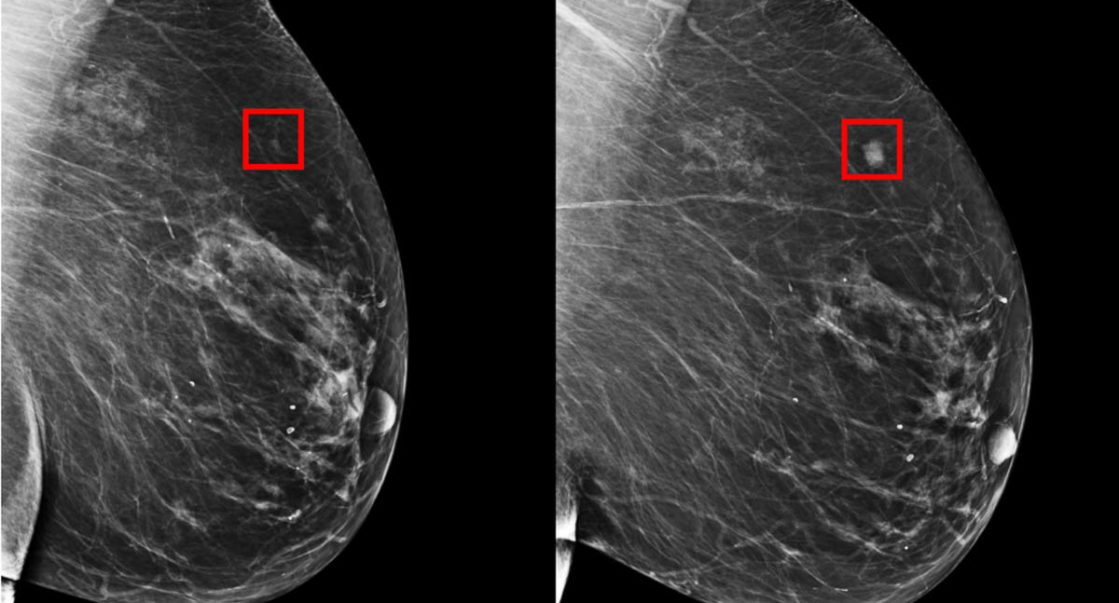
\includegraphics[width=\textwidth]{cancer}
  \vfill
\end{frame}

{
  \setbeamercolor*{background canvas}{bg=white}
  \setbeamercolor{normal text}{fg=black}
  \usebeamercolor[fg]{normal text}
  
  \begin{frame}[t, c]{Mieux comprendre le cerveau}{}
    \vfill
    \centering
    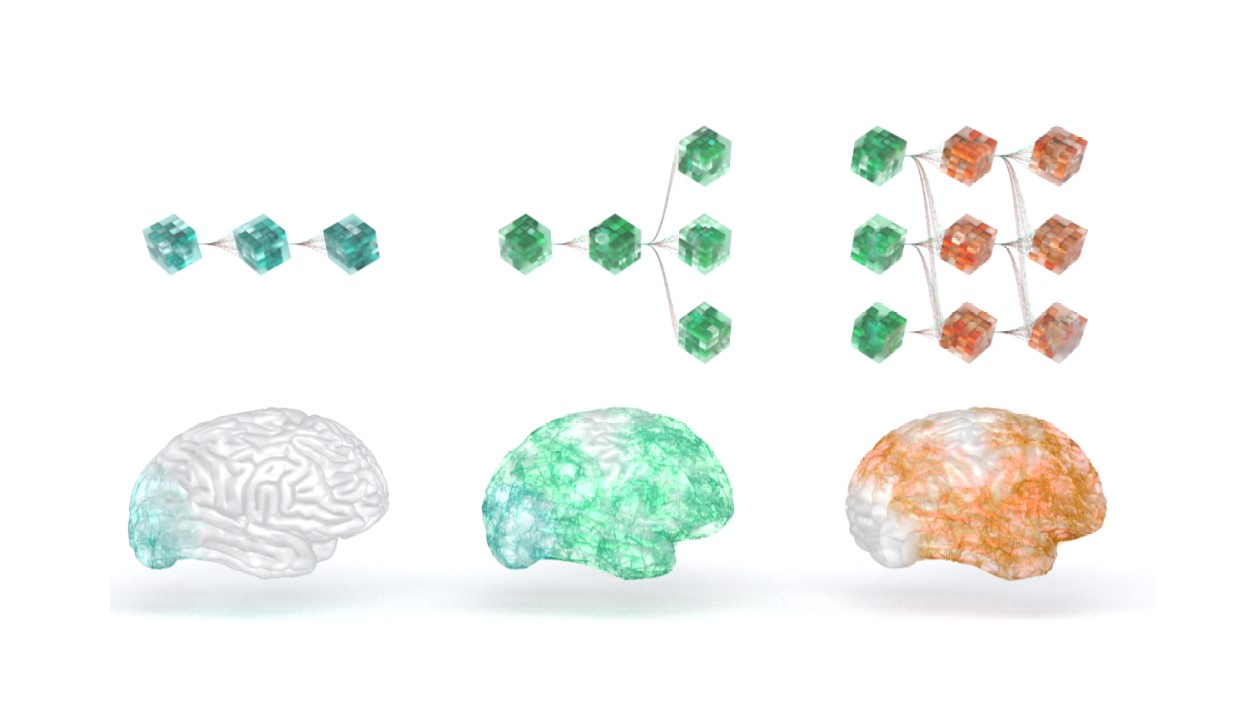
\includegraphics[width=\textwidth]{meta_brain}
    \vfill
  \end{frame}

\begin{frame}[t, c]{Identifier des modèles physiques}{}
  \centering
  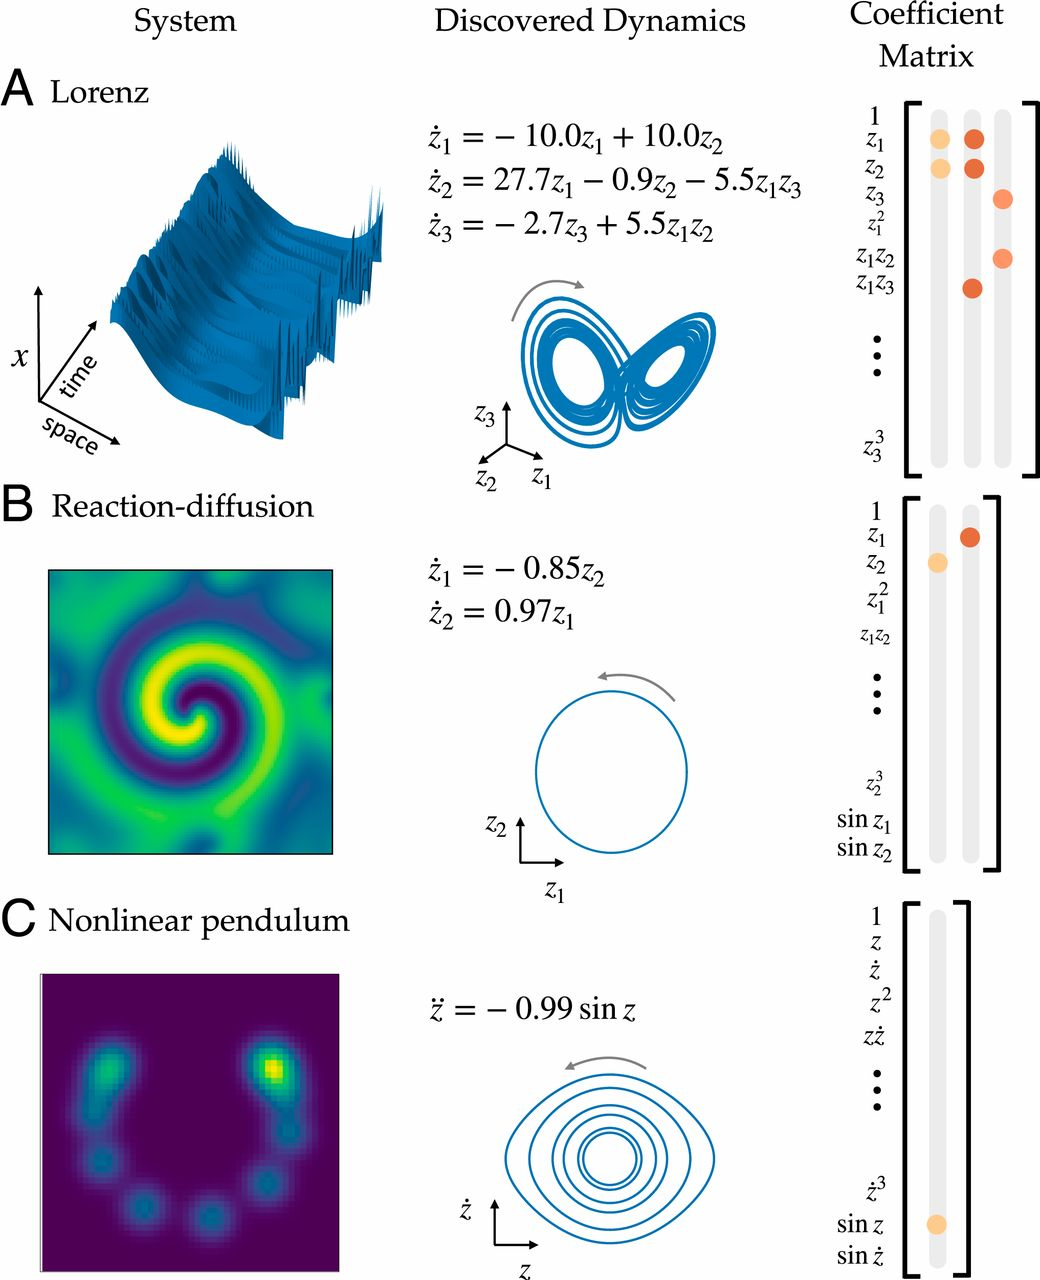
\includegraphics[height=.8\textheight]{sindy}
\end{frame}

}


\section{Le mot de la fin}
\begin{frame}
  \sectionpage
\end{frame}

{
  \setbeamercolor*{background canvas}{bg=white}
  \setbeamercolor{normal text}{fg=black}
  \usebeamercolor[fg]{normal text}


  \begin{frame}
    \centering
    \vfill
    \movie[externalviewer]{
\includegraphics[width=.25\textwidth]{play_button}}{imgs/robot_fail.mov}
    \vfill
  \end{frame}


  \begin{frame}
    \begin{minipage}{.28\textwidth}
      \centering
      
\includegraphics[height=.15\textheight]{github}
    \end{minipage}%
    \hfill
    \begin{minipage}{.68\textwidth}
      \url{https://loiseaujc.github.io/}
    \end{minipage}

    \bigskip

    \begin{minipage}{.28\textwidth}
      \centering
      
\includegraphics[width=\textwidth]{medium}
    \end{minipage}%
    \hfill
    \begin{minipage}{.68\textwidth}
      \url{https://loiseau-jc.medium.com/}
    \end{minipage}

    \bigskip

    \begin{minipage}{.28\textwidth}
      \centering
      
\includegraphics[height=.15\textheight]{twitter}
    \end{minipage}%
    \hfill
    \begin{minipage}{.68\textwidth}
      \url{@loiseau_jc}
    \end{minipage}

  \end{frame}
}
%%%%%
%%%%%
%%%%%     SLIDE FINALE
%%%%%
%%%%%


\begin{frame}
  \vfill
  \flushright

  {
  \Large
  \textbf{Merci de votre attention !}
  }

  \bigskip

  {
  \large
  \textcolor{gray}{
  \textbf{Des questions?}
  }
  }
  \vfill
\end{frame}

\end{document}
